\chapter{Discretisation Convergence}\label{ch:appendix-convergence}

\begin{figure}[ht]
  \centering
  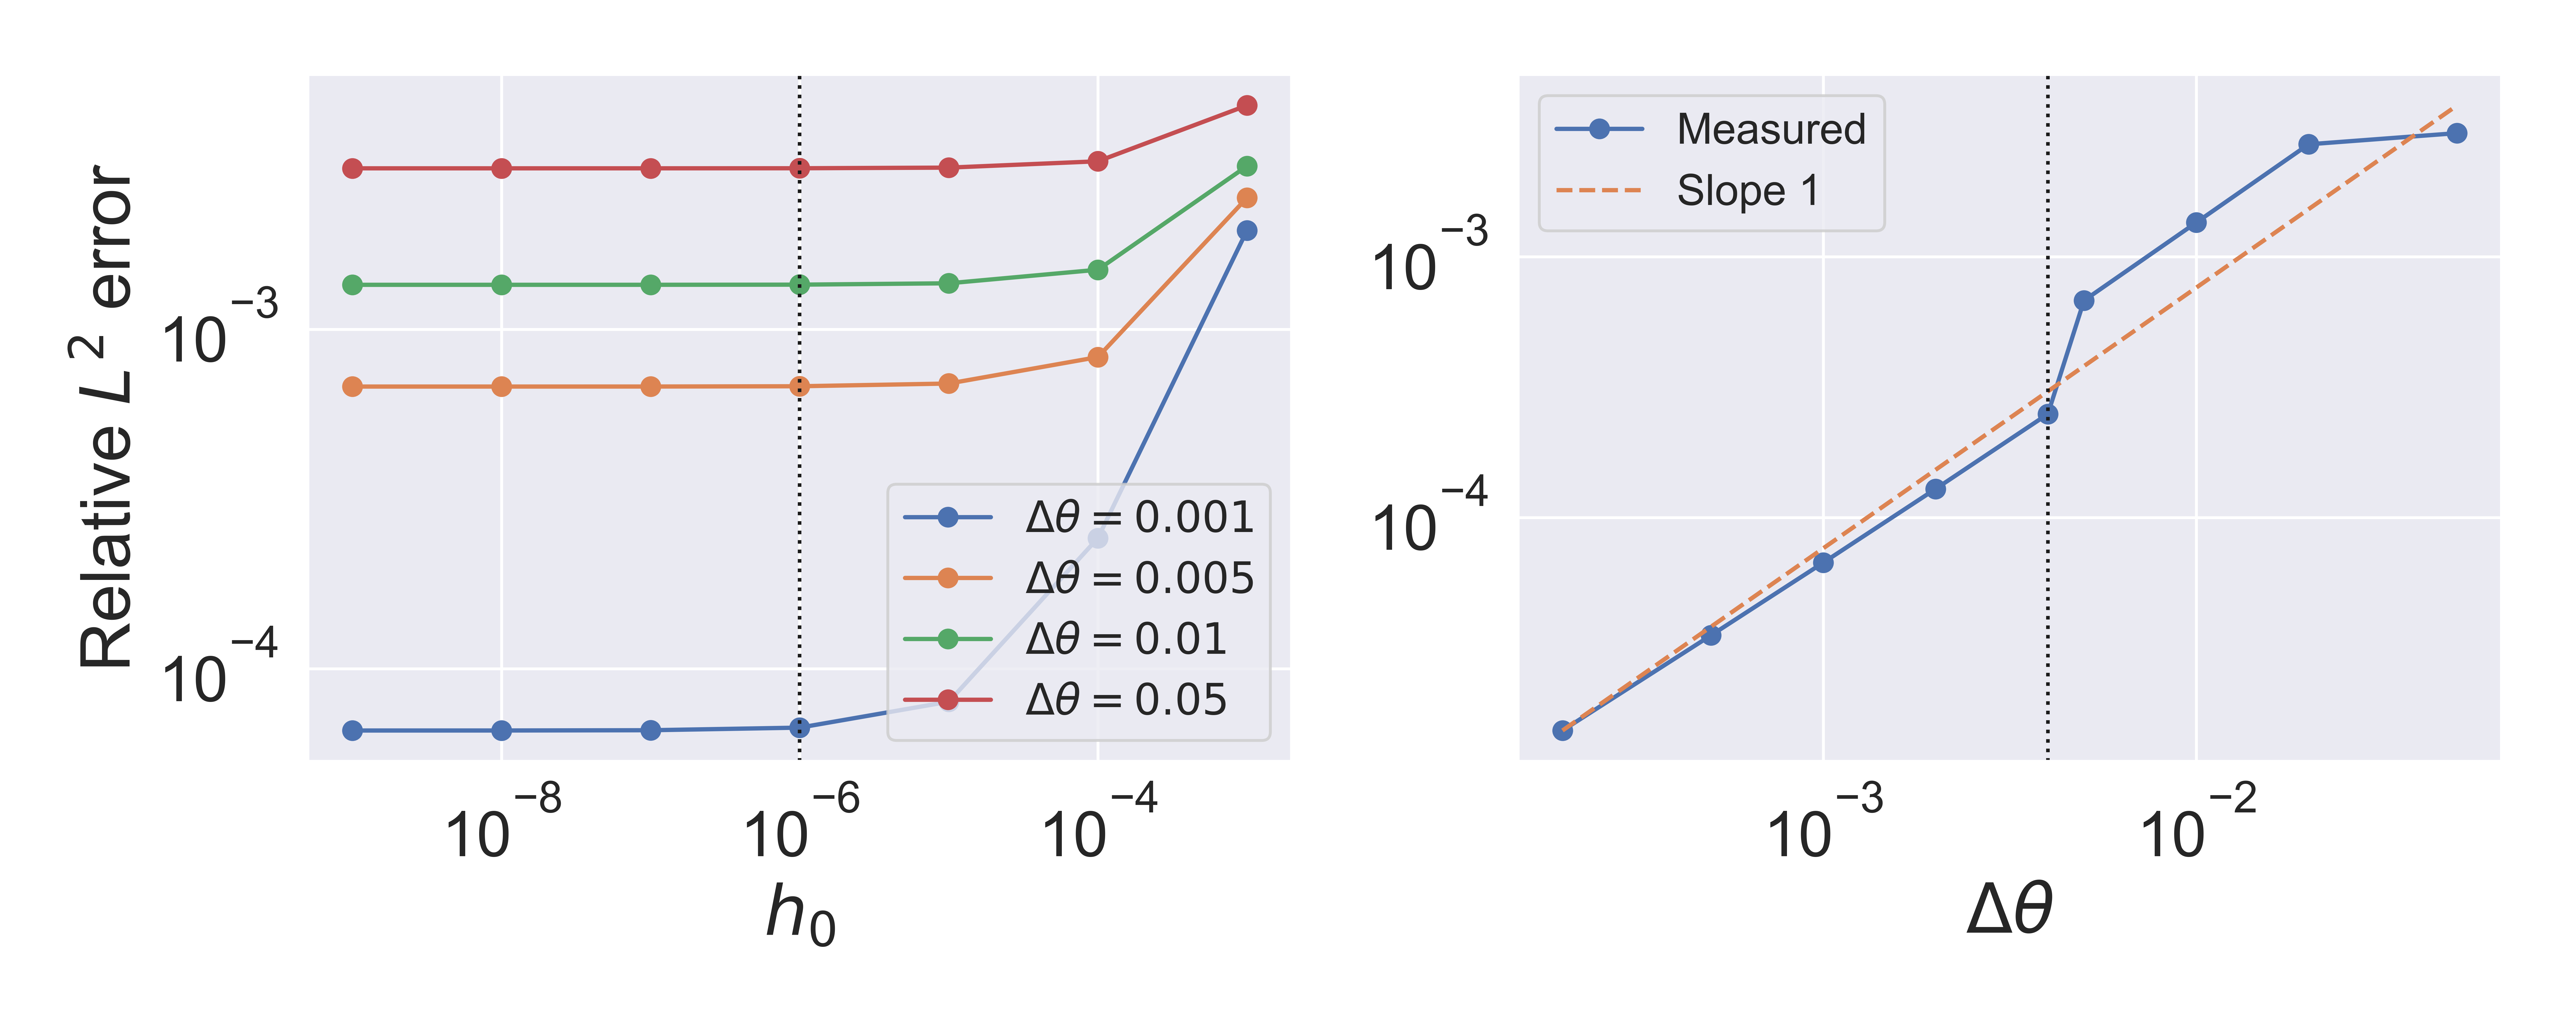
\includegraphics[width=1.00\textwidth]{figures/7-discretisation.png}
  \caption[Convergence of the heterogeneous solver]{Convergence of the
    heterogeneous solver. Relative $L^2$ error of the simulated current
    against a reference solution. Left: spatial refinement at four fixed
    $\Delta\theta$; the error plateaus for $h_0 \lesssim 10^{-6}$.
    Right: temporal refinement at $h_0 = 10^{-6}$; the measured slope
    matches the first-order backward Euler rate. Dotted lines mark the
  adopted values $h_0 = 10^{-6}$ and $\Delta\theta = 4 \times 10^{-3}$.}
\end{figure}

\begin{figure}[ht]
  \centering
  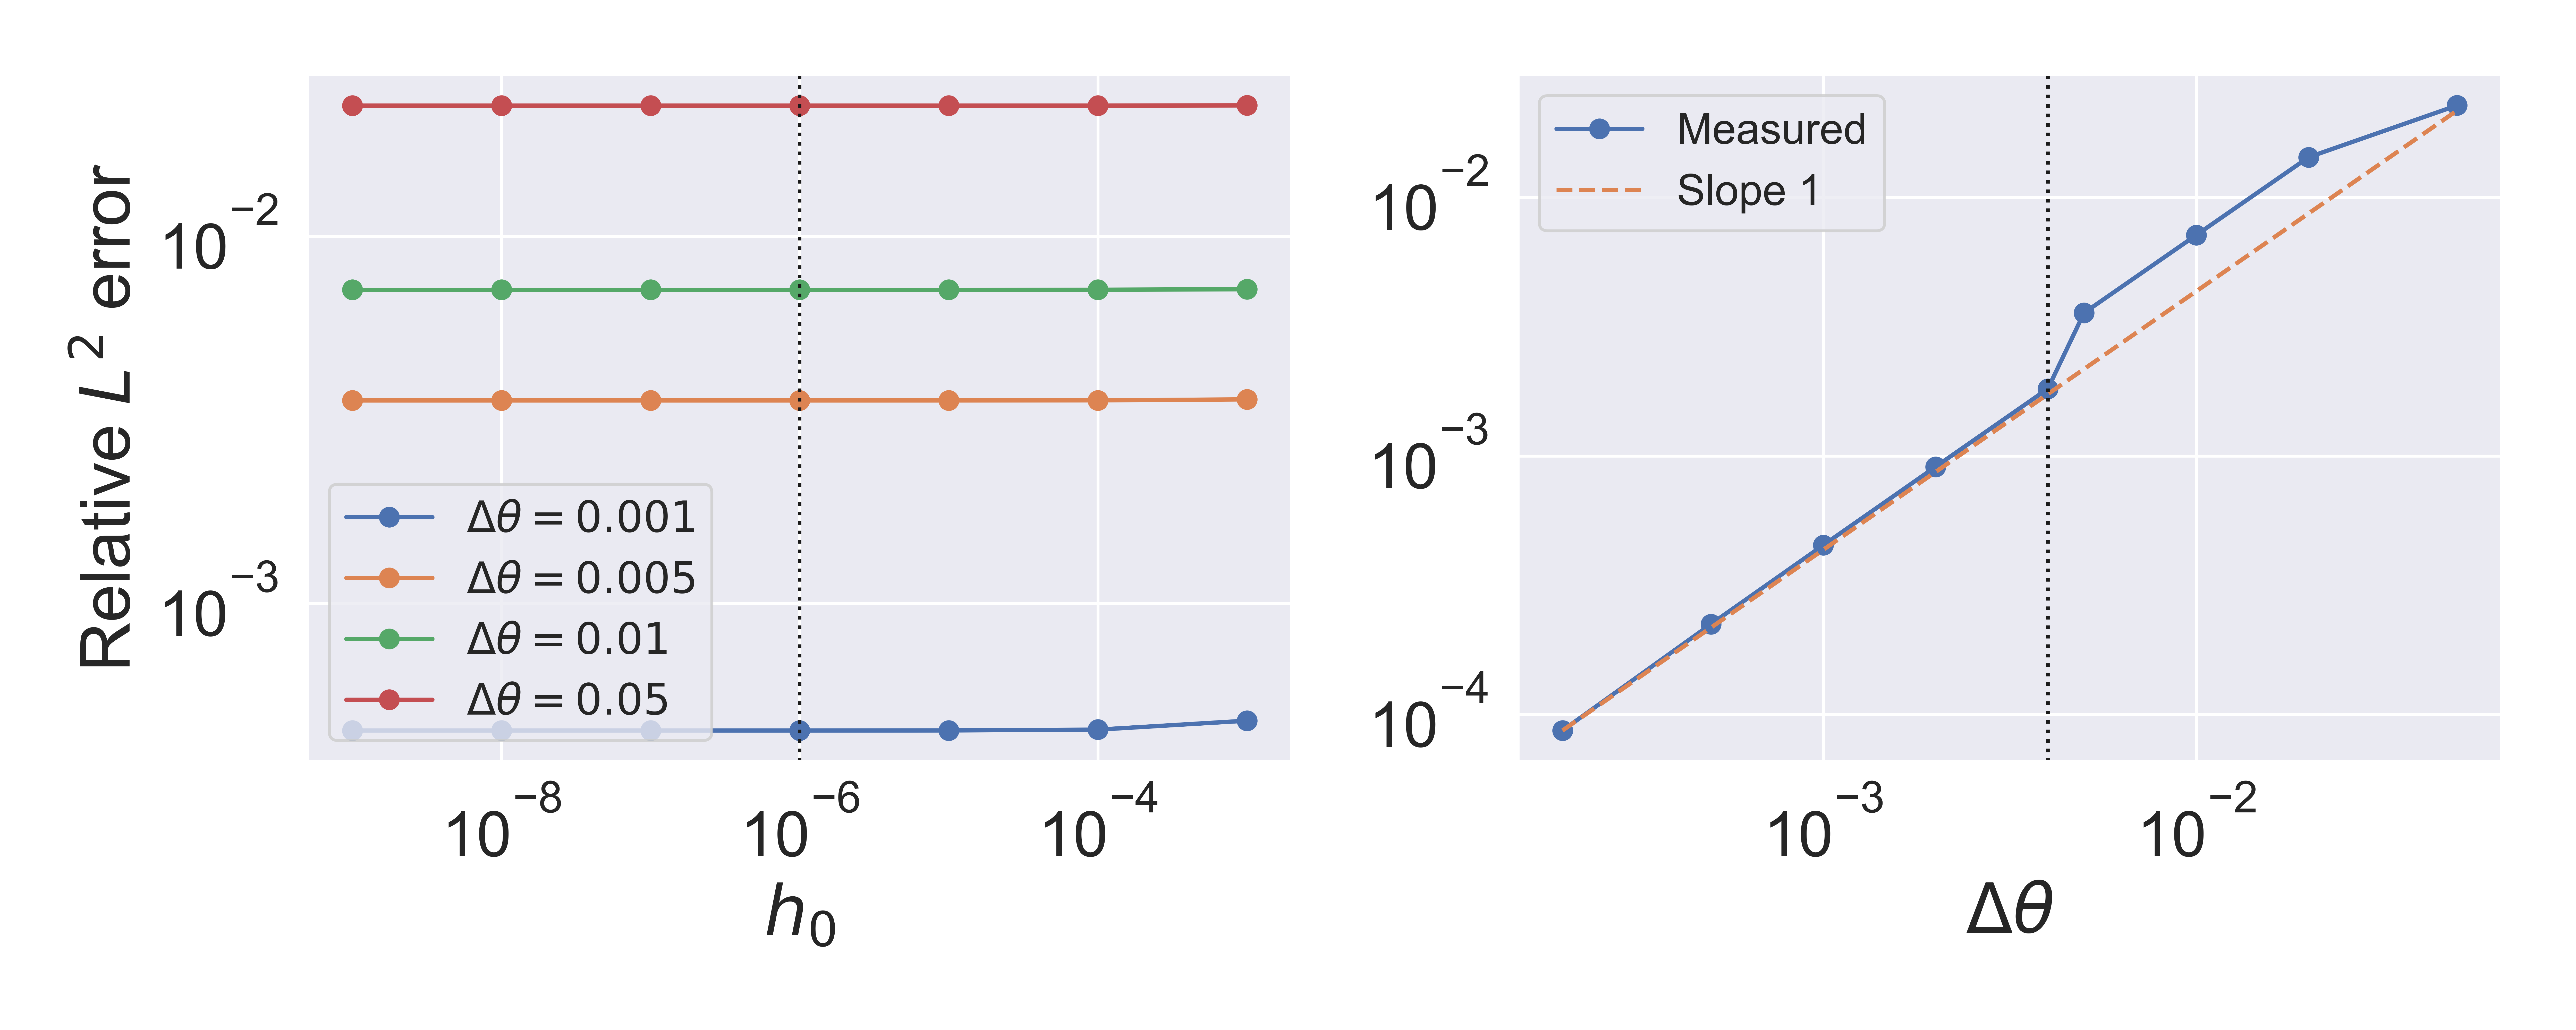
\includegraphics[width=1.00\textwidth]{figures/8-discretisation.png}
  \caption[Convergence of the adsorption solver]{Convergence of the
    adsorption solver against a Newton--Raphson reference solution.
    Left: spatial refinement at four fixed $\Delta\theta$; the error
    is insensitive to $h_0$ across the range tested, indicating that
    the temporal error dominates. Right: temporal refinement at $h_0 =
    10^{-6}$; the measured slope matches the first-order backward Euler
    rate. Dotted lines mark the adopted values $h_0 = 10^{-6}$ and
  $\Delta\theta = 4 \times 10^{-3}$.}
\end{figure}
